\documentclass{article}

%% PAQUETES

% Paquetes generales
\usepackage[margin=2cm, paperwidth=210mm, paperheight=297mm]{geometry}
\usepackage[spanish]{babel}
\usepackage[utf8]{inputenc}
\usepackage{gensymb}

% Paquetes para estilos
\usepackage{textcomp}
\usepackage{setspace}
\usepackage{colortbl}
\usepackage{color}
\usepackage{color}
\usepackage{upquote}
\usepackage{xcolor}
\usepackage{listings}
\usepackage{caption}
\usepackage[T1]{fontenc}
\usepackage[scaled]{beramono}

% Paquetes extras
\usepackage{amssymb}
\usepackage{float}
\usepackage{graphicx}
\usepackage{url}
\usepackage{enumerate}
\usepackage{color}

%% Fin PAQUETES


% Definición de preferencias para la impresión de código fuente.
%% Colores
\definecolor{gray99}{gray}{.99}
\definecolor{gray95}{gray}{.95}
\definecolor{gray75}{gray}{.75}
\definecolor{gray50}{gray}{.50}
\definecolor{keywords_blue}{rgb}{0.13,0.13,1}
\definecolor{comments_green}{rgb}{0,0.5,0}
\definecolor{strings_red}{rgb}{0.9,0,0}

%% Caja de código
\DeclareCaptionFont{white}{\color{white}}
\DeclareCaptionFont{style_labelfont}{\color{black}\textbf}
\DeclareCaptionFont{style_textfont}{\it\color{black}}
\DeclareCaptionFormat{listing}{\colorbox{gray95}{\parbox{16.78cm}{#1#2#3}}}
\captionsetup[lstlisting]{format=listing,labelfont=style_labelfont,textfont=style_textfont}

\lstset{
	aboveskip = {1.5\baselineskip},
	backgroundcolor = \color{gray99},
	basicstyle = \ttfamily\footnotesize,
	breakatwhitespace = true,   
	breaklines = true,
	captionpos = t,
	columns = fixed,
	commentstyle = \color{comments_green},
	escapeinside = {\%*}{*)}, 
	extendedchars = true,
	frame = lines,
	keywordstyle = \color{keywords_blue}\bfseries,
	language = Oz,                       
	numbers = left,
	numbersep = 5pt,
	numberstyle = \tiny\ttf
amily\color{gray50},
	prebreak = \raisebox{0ex}[0ex][0ex]{\ensuremath{\hookleftarrow}},
	rulecolor = \color{gray75},
	showspaces = false,
	showstringspaces = false, 
	showtabs = false,
	stepnumber = 1,
	stringstyle = \color{strings_red},                                    
	tabsize = 2,
	title = \null, % Default value: title=\lstname
	upquote = true,                  
}

%% FIGURAS
\captionsetup[figure]{labelfont=bf,textfont=it}
%% TABLAS
\captionsetup[table]{labelfont=bf,textfont=it}

% COMANDOS

%% Titulo de las cajas de código
\renewcommand{\lstlistingname}{Código}
%% Titulo de las figuras
\renewcommand{\figurename}{Figura}
%% Titulo de las tablas
\renewcommand{\tablename}{Tabla}
%% Referencia a los códigos
\newcommand{\refcode}[1]{\textit{Código \ref{#1}}}
%% Referencia a las imagenes
\newcommand{\refimage}[1]{\textit{Imagen \ref{#1}}}


\begin{document}
\pagenumbering{roman}
\setcounter{page}{5}

% TÍTULO, AUTORES Y FECHA
\begin{titlepage}
	\vspace*{\fill}
	\begin{center}
		\Large 75.06 Organización de Datos \\
		\Huge TP N°1: Catálogo discográfico \\
		\bigskip\huge\textit{Grupo 07} \\
		\bigskip\bigskip\bigskip\bigskip\bigskip\bigskip
		\bigskip\bigskip\bigskip\bigskip\bigskip\bigskip\bigskip
		\medskip\huge\textit{``Documentación de diseño''} \\
		\date{}
	\end{center}
	\vspace*{\fill}
\end{titlepage}
\newpage



% ÍNDICE
\tableofcontents
\newpage
\pagenumbering{arabic}


% INTRODUCCIÓN
\section{Introducción}
	
	El siguiente documento tiene como objetivo especificar y precisar los detalles técnicos de la realización de la primera parte del trabajo práctico. Se explican los problemas surgidos a la hora del diseño y las soluciones encaradas para solventar los mismos.
	\par
	Todos los archivos y códigos fuente aquí mencionados y relacionados al proyecto, así como también el presente informe, pueden ser encontrados y descargados del repositorio del grupo (\url{https://github.com/federicomrossi/7506-tp-grupo07}).
\bigskip




% REQUERIMIENTOS PLANTEADOS
\section{Requerimientos planteados}

	El trabajo solicitado se basa en la creación de un sistema para la generación de un catalogo a partir de archivos de letras de canciones de diversos autores. Dicho sistema debe ser capaz de realizar búsquedas por autor, titulo y frases, entregando como resultado los temas que coincidan con los parámetros ingresados.
	\par
	A su vez se exigieron ciertas condiciones para la realización del trabajo a la hora del manejo de las estructuras. El índice para la búsqueda por titulo debía estructurarse como un hash, por autor como un árbol B+ y los archivos de texto como bloques de registros variables.
	\par
	El producto final es una aplicación de consola que permite realizar las operaciones pedidas.
	\bigskip




% DIVISION DEL TRABAJO
\section{División del trabajo}

	El trabajo esta divido en tres capas funcionales: la física, la lógica y el front-end.
	\par
	A su vez, la capa lógica esta formada por tres módulos principales, a saber, el árbol B+, el hash extensible y las estructuras de recuperación de textos. La distribución mencionada se puede observar en la \textit{Figura 1}.
	\bigskip\medskip


% Figura 1
\begin{figure}[h]
	\centering
	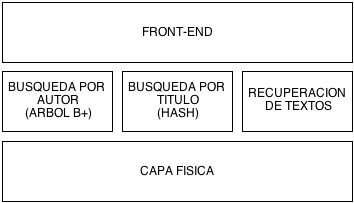
\includegraphics[width=0.48\textwidth]{images/DivisionModulos.png}
	\medskip
	\caption{Esquema de la estructuración en capas.}
\end{figure}
\bigskip\smallskip


	Esta división esta fundamentada en tener el menor acoplamiento posible entre las clases y sobretodo entre los módulos lógicos. A su vez, permite una fácil división de las tareas entre los integrantes del grupo de trabajo.
	\medskip




% DETALLES TECNICOS: 1ra Parte
\section{Detalles técnicos: \textit{1ra Parte}}

	A continuación se describirá con un mayor nivel de detalle cada uno de los módulos que componen el sistema en esta primer etapa del proyecto. \\


% DETALLES TECNICOS - Capa Física
\subsection{Capa Física}
	
	La capa física de este trabajo se centra alrededor de dos clases: \textit{ArchivoBloques} y \textit{SerialBuffer}.
	\par	
	La primera es la encargada de la interacción directa con el disco. La misma define interfaces para poder leer y escribir un archivo en función de bloques de un tamaño fijo y parametrizable.
	\par
	El problema que surgió aquí es que independientemente de utilizar el modo normal de apertura para escribir de C++ (ios::out), el archivo era truncado y se perdía su contenido, quedando solamente el último bloque escrito. La solución para esto fue que si se quería modificar un bloque ya existente, se utilizara un archivo de trabajo temporal para pasar el contenido original, intercalar el bloque a modificar y luego copiar el resto del archivo. Posteriormente se elimina el archivo original y se renombra el de trabajo. Debido a que esto es muy costoso y generalmente muchas de las operaciones de escritura consisten en agregar un nuevo bloque al final, existe un método que abre el archivo en modo append (ios::app) y agrega el nuevo bloque. La lectura en cambio no presento problema alguno.
	\par
	SerialBuffer es la clase encargada de brindar los medios para poder persistir de manera ordenada los registros de cada estructura. La misma presenta dos métodos principales, pack y unpack.
	\par
	El primero se encarga de agregar registros a un buffer de caracteres (cabe aclarar que se escogió por archivos de tipo binario para la persistencia de datos). Para poder recuperar la información a posteriori, antes de empaquetar cada registro carga en el buffer un prefijo de longitud para poder saber cuanto va a tener que recuperar del buffer a un objeto.
	\par
	El segundo, hace el trabajo inverso y restaura la información de un buffer, que previamente se leyó desde el disco, a un objeto. Utiliza el prefijo de longitu para saber la cantidad de caracteres a pasar desde el buffer al objeto de destino.
	\par
	Como puede notarse, el buffer es la estructura fundamental y puede verse al mismo como una sucesión de registros como la siguiente:
	\bigskip


	{\ttfamily\footnotesize
	[prefijoLongitud(unsigned short int), reg(registro genérico de longitud variable)] \\}
	\medskip


	Donde el tamaño total queda comprendido dentro del tamaño del buffer.
	\par
	Una carácteristica de esta implementación es la relación uno a uno que debe haber entre los tamaños de bloque y de los buffer, ya que si los mismos no coincidieran generarían errores de segmentación a la hora de tratar datos en memoria.	
	\bigskip\medskip




% DETALLES TECNICOS - Arbol B+
\subsection{Árbol B$^+$}
\medskip

	Una de las estructuras mas importantes de la aplicación es el Árbol B$^+$, siendo esta la base sobre la cual se sostiene el sistema de indexación. Su implementación consta de una clase central denominada \textit{ArbolBmas} y de tres estructuras secundarias denominadas \textit{Nodo}, \textit{NodoInterno} y \textit{NodoHoja}. Como puede sospecharse, las dos últimas estructuras heredan de \textit{Nodo}, siendo esta la estructura padre. El sentido de este diseño es establecer métodos comunes de manera tal de poder aplicar polimorfismo sobre ellas desde la clase \textit{ArbolBmas}. Más detalles sobre los nodos serán expuestos en los siguientes apartados de la sección.
	\par
	El árbol se almacenará en un archivo de bloques fijos, en el cual se aparta el primer bloque (bloque cero) para poder almacenar la metadata del mismo. Esta consta del \textit{nivel} máximo que posee (si existen los niveles 0, 1 y 2, se almacenará el valor 2), un \textit{contador de bloques} existentes el cual toma registro del último bloque asignado de manera tal de poder proveer un nuevo bloque en una inserción posterior, y el \textit{número de bloque de la raíz}. Este último sirve para poder cargar la raiz al abrir el árbol, es decir, la raíz se encontrará siempre en memoria. Como puede notarse, a consecuencia de esto último, el bloque raíz no es siempre el mismo, sino que variará a medida que el árbol vaya creciendo y sea necesario realizar particiones de nodos. Se decidió hacerlo de esta manera a fin de poder reducir las lecturas y evitar las transformaciones entre tipos de nodos (ya que en un principio, cuando el árbol se encuentre vació, la raíz será un nodo hoja, pero si es partida, se convertirá en un nodo interno).
\bigskip



% DETALLES TECNICOS - Arbol B+ - Nodos internos y nodos hoja
\subsubsection{Nodos internos y nodos hoja}
	
	Cada nodo esta representado por un bloque en el archivo, en el cual se guardarán claves en el caso de los nodos internos, y registros en nodos hoja. La determinación de cuantas claves o registros caben en los nodos se realiza tomando en cuenta el tamaño del bloque especificado por el usuario en el archivo de configuración. 
	\par
	Una de las problemáticas a resolver fue cómo determinar el overflow, para lo cual se decidió separar una clave o registro en cada bloque que cumpla la función de posición de overflow. Es decir, al ingresar elementos en un nodo, una vez que se llega a ocupar la posición de overflow, el nodo lo advierte y da aviso de tal evento a su nodo padre. Este comportamiento se logró devolviendo un valor ĺógico en el método \textit{insertar()} de los nodos, siendo que, la devolución de \textit{false} significa que el nodo no está en overflow y un retorno del valor lógico \textit{true} implica que el nodo se encuentra sobrecargado.
	\par
	Cada nodo, además, provee a su padre un método que permite realizar la división con un nodo hermano. Este método se denomina \textit{dividir()}. Entonces, en caso de que un nodo entre en overflow, su padre deberá crear otro nodo que sea del mismo tipo que el primero, y pasárselo como parámetro al método \textit{dividir} de aquel que se encuentra sobrecargado. De esta manera se realizará la partición que permitirá volver a un estado estable al árbol.
	\par
	Otro detalle a tener en cuenta es que para poder persistir o leer los nodos, existen los métodos \textit{guardar()} y \textit{cargar()} respectivamente. Estos guardarán o cargarán desde el número de bloque que se encuentra asignado al objeto de tipo \textit{Nodo}.
\bigskip



% DETALLES TECNICOS - Arbol B+ - Registros genéricos
\subsubsection{Registros genéricos}
	
	Una restricción importante que posee el árbol es que los registros a insertarse deben ser, por contrato, objetos de tipos que hereden de la clase \textit{RegistroGenerico}. Por contrato nos referimos a que el árbol puede llegar a aceptar otros objetos de diferentes tipos, pero el comportamiento ante estos puede ser inestable debido a la necesidad de contar con ciertos métodos primordiales. Esta decisión de diseño se debe a la forma en que internamente se encuentran organizados los registros al momento de ser cargados en memoria.
	\par
	Además, debe tenerse en cuenta que dichos tipos descendientes de \textit{RegistroGenerico} deben sobrecargar los métodos de serialización para, de esta manera, poder lograr un correcto funcionamiento del árbol.
	\par
	De todas maneras, la gran ventaja es que el uso de registros genéricos le da la posibilidad al usuario de poder almacenar todo aquello que desea en el árbol, pudiéndose hacer uso de este último en distintos tipos de implementaciones.
\bigskip



% DETALLES TECNICOS - Arbol B+ - Contenedor ListaFija
\subsubsection{Depuración}

	Al iniciar el diseño, se tuvo que pensar en una forma de realizar las pruebas, de manera tal de poder constatar el correcto funcionamiento del árbol. Es por esto que a los nodos se les ha agregado el método \textit{imprimir()}, el cual debe imprimir por salida estándar una representación de su contenido manteniendo un formato predeterminado. Para el caso de nodos hoja el formato es el siguiente:
	\bigskip

	{\ttfamily\footnotesize
	[nivel], [numero\_bloque]: ([clave1])..([claveN])[nodo\_hermano], \\}

	mientras que para los nodos internos el formato es:
	\bigskip

	{\ttfamily\footnotesize
	[nivel], [numero\_bloque]: [hijo1]([clave1])[hijo2]([clave2])..[hijoN]([claveN])[hijoN+1]. \\}

	La clase \textit{ArbolBmas} también posee un método \textit{imprimir()}, el cual invoca al método \textit{imprimir()} del nodo ubicado en la raíz.
	\par
	Los nodos internos, aparte de imprimirse a sí mismos, también invocan a los \textit{imprimir()} de sus hijos, generándose así, en la salida estándar, una representación completa del árbol. Esto permite hacer sencillo seguimiento de las inserciones, particiones, etc.
\bigskip\medskip



% DETALLES TECNICOS - Hash Extensible
\subsection{Hash Extensible}
\medskip

	Para la implementación del \textit{Hash Extensible} se buscó poder modularizar lo más posible las estructuras que hacen a su funcionamiento.Estas son el \textit{Block}, perteneciente a la capa física, y \textit{BlockTable} y \textit{HashExtensible}, pertenecientes a la capa lógica.
	\par
	\textit{HashExtensible} cumple el trabajo de función de dispersión, es decir, dado un ID y aplicando una función de dispersión, genera otro valor, utilizado para ver donde ubicar dicho ID.
	\par
	\textit{BlockTable} y \textit{Block} son las estructuras pilares en el funcionamiento de esta estructura.
	\par
	Empezando por la estructura más baja se encuentra \textit{Block}, también llamada \textit{Buckets} (Cubetas). Su misión es la de contener registros, pero al ser de un tamaño fijo, se pueden llenar y provocar problemas los cuales son analizados más adelante. Los bloques cuentan además con un número de bloque por el cual son referenciados y un llamado tamaño de dispersión (TD). Este número representa la cantidad de veces que un bloque es referenciado por la tabla y es calculado como
	\medskip

	\begin{center}
	$TD = {TT \over N_i}$
	\end{center}
	\medskip

	donde \textit{TT} es el tamaño de la tabla y \textit{N$_i$} la cantidad de veces que es referenciado el bloque \textit{i} por la tabla.
	\par
	Las cubetas están organizadas por una clase lógica, \textit{BlockTable}, que contiene un arreglo con un número (siempre potencia de 2) de estas. Esta clase es la encargada de manejar el comportamiento del hash, haciendo que este sea extensible.
	\par
	Cuando un bloque se desborda, la tabla duplica su tamaño, copiándose a sí misma en la segunda mitad, generando así varias referencias a los mismos bloques (estos siguen conservando su tamaño de dispersión).
	\par
	Tanto \textit{Block} como \textit{BlockTable} son persistidas en un archivo de bloques y en un archivo secuencial respectivamente. Se eligió usar un archivo secuencial ya que teóricamente el arreglo de bloques no suele tomar números incontrolables en memoria, sino unos pocos bytes.
	El flujo para agregar un registro es el siguiente:
	\bigskip


	{\ttfamily\footnotesize
	\begin{enumerate}
	\itemsep=5pt \topsep=0pt \partopsep=0pt \parskip=0pt \parsep=0pt

		\item Se aplica una función de dispersión, obteniendo así la posición en la tabla de bloques (BlockTable) donde se ubicaría el registro.

		\item En dicha posición se encuentra un número de bloque dado. 

		\item Se busca el bloque en el archivo de bloques y se lo trae a memoria.

		\item Una vez bufferizado, se verifica si hay tamaño para agregar un nuevo registro. 

		\item Si hay tamaño:
			\begin{enumerate}
			\itemsep=5pt \topsep=0pt \partopsep=0pt \parskip=0pt \parsep=0pt

				\item se agrega el bloque al buffer. 

			\end{enumerate}

			Sino, se presentan dos claras situaciones:

			\begin{enumerate}
			\itemsep=5pt \topsep=0pt \partopsep=0pt \parskip=0pt \parsep=0pt

				\item Si TD = TT (es el caso en que el bloque está siendo referenciado una sola vez):
					
					\begin{enumerate}
					\itemsep=5pt \topsep=0pt \partopsep=0pt \parskip=0pt \parsep=0pt

						\item Se duplica la tabla.
						\item Se crea un nuevo bloque.
						\item Se lo agrega en la posición donde estaba el bloque anterior, mientras que el viejo queda en la segunda parte de la tabla.
						\item Se redispersan los registros ( aplica la función hash ) entre el bloque viejo y el nuevo bloque.
						\item Se agrega el registro en el bloque correspondiente.

					\end{enumerate}

				\item Si TD != TT (el bloque está referenciado más de una sola vez):

					\begin{enumerate}
					\itemsep=5pt \topsep=0pt \partopsep=0pt \parskip=0pt \parsep=0pt

						\item Se crea un bloque 
						\item Se lo inserta en la posición donde estaba el bloque viejo y en las siguientes TD posiciones a su derecha y TD posiciones a su izquierda.
						\item Se redispersan los registros.
						\item Se agrega el registro en el bloque correspondiente.

					\end{enumerate}
			\end{enumerate}

		\item Se persiste el buffer en memoria.

		\item Una vez finalizado el proceso de inserción de registros, se persiste la tabla en el archivo secuencial.

	\end{enumerate}}
	\bigskip\bigskip

	Para la búsqueda el proceso es mucho más sencillo:
	\bigskip

	{\ttfamily\footnotesize
	\begin{enumerate}
	\itemsep=5pt \topsep=0pt \partopsep=0pt \parskip=0pt \parsep=0pt

		\item Se aplica una función de dispersión, obteniendo así la posición en la tabla de bloques (BlockTable) donde se ubicaría el registro.

		\item En dicha posición se encuentra un número de bloque dado.

		\item Se busca el bloque en el archivo de bloques y se lo trae a memoria.

		\item Una vez bufferizado, se serializan los registros y se busca secuencialmente por el deseado.

	\end{enumerate}}
\bigskip\medskip




% DETALLES TECNICOS - Indexacion
\subsection{Indexación}
\medskip

	La indexación de un tema fue dividida en tres partes. Un índice de títulos, implementado en la clase ``\textit{IndiceTitulo}'', un índice de autores, implementado en la clase ``\textit{IndiceAutor}'' y un un índice de Recuperacion de texto, implementado en la clase ``\textit{RTTgenerator}''.
\bigskip



% DETALLES TECNICOS - Indexacion - Indice de Autor
\subsubsection{Índice de Autor}
\medskip

	El mismo esta basado en un Árbol B$^+$. En este último se almacenan registros con el formato 
	\bigskip

	{\ttfamily\footnotesize
	(idAutor, clave1, clave2, clave3, clave4, clave5, refLista) \\}

	Las claves representan referencias a posiciones de canciones en el archivo maestro. La ``\textit{refLista}'' representa una referencia a una posicion al archivo de listas de autores. Se eligio esta solucion ya que es factible que existan muchas canciones del mismo autor.
\bigskip



% DETALLES TECNICOS - Indexacion - Indice de Autor
\subsubsection{Índice de Título}
\medskip

	El mismo esta basado en un Hash Extensible. En el mismo se almacenan registros con el formato 
	\bigskip

	{\ttfamily\footnotesize
	(idTitulo, clave1, clave2, clave3, refLista) \\}

	Las claves representan referencias a posiciones de canciones en el archivo maestro. La ``\textit{refLista}'' representa una referencia a una posición al archivo de listas de títulos. Se eligió esta solución ya que, si bien es poco probable, podría suceder que existan muchas canciones con el mismo título.
\bigskip



% DETALLES TECNICOS - Indexacion - Indice de RTT
\subsubsection{Índice de RTT}
\medskip

	El mismo esta principalmente basado en un Árbol B$^+$. Además se tienen archivos auxiliares para guardar las listas invertidas de documentos y posiciones.
	\par
	En el árbol se guardan registros con el formato
	\bigskip

	{\ttfamily\footnotesize
	(idPalabra, refListaDocs) \\}
	 
	En el archivo de listas de documentos se guardan registros con el formato
	\bigskip

	{\ttfamily\footnotesize
	(idDoc, refListaPos) \\}
	
	En el archivo de listas de posiciones se guardan las posiciones donde aparece dicho término.
	\par
	Cuando se quiere resolver una consulta primero se busca en el árbol todas las listas de documentos. Se intersectan las mismas para obtener aquellos documentos donde aparezcan todos los términos. Por último, utilizando el archivo de posiciones se verifica que las posiciones relativas de la consulta sean las mismas que las posiciones relativas en el archivo original.
\bigskip\bigskip




% DETALLES TECNICOS: 2da Parte
\section{Detalles técnicos: \textit{2da Parte}}

	A continuación se describirá con un mayor nivel de detalle cada uno de los módulos que componen el sistema en esta segunda etapa del proyecto. \\



% DETALLES TECNICOS - Compresion
\subsection{Compresión}
\medskip

	La compresión de los temas fue realizada mediante una implementación del algoritmo PPMC. El mismo fue subdivido en dos módulos para su realización: el correspondiente a la compresión/descompresión aritmética (implementado en la clase ``\textit{Aritmetico}'') y el de la predicción (implementado en la clase ``\textit{Contexto}'' y sus herederas). A continuación un detalle de ambos.
\bigskip



% DETALLES TECNICOS - Compresion - Aritmetico
\subsubsection{Aritmético}
\medskip

	La implementación del mismo se realizó siguiendo la teoría desarrollada en clase. Sus parametros son la probabilidad del caracter a comprimir/descomprimir, la probabilidad acumulada y la probabilidad total. 

\bigskip



% DETALLES TECNICOS - Compresion - Predictor
\subsubsection{Predictor}
\medskip

	Este caso requirió de mayor planeamiento debido a la escasa bibliografía con respecto a la implementación de este aspecto del PPMC. A diferencia del resto del diseño, para esta parte se decidió realizar una planificación conjunta, llegando a la siguiente realización. Debido a las particularidades de cada uno de los ordenes divisamos tres tipos distintos, representados por las clases ``\textit{CtxM1}'', ``\textit{Ctx0}'' y ``\textit{CtxN}''. La estructura principal del predictor es una lista enlazada, cuyos nodos representan cada uno de los ordenes con los cuales se esta trabajando.
	\par
	Las carácteristicas de los ordenes -1 y 0, permitían generar las estrúcturas para almacenar los contextos de manerar estática (desde el punto de vista de la alocación de la memoria). En particular, el orden -1 se maneja con un simple contador para representar la probabilidad total y se va decrementando según el resultado de las exclusiones, es decir, que la probabilidad de los caracteres se obtiene de manera implícita. Para el caso del orden 0, las probabilidades se alojan en un arreglo de 257 posiciones. Debido a que esto genera un bajo overhead de memoria pero, permite acceso O(1) a todas las probabilidades, fue el camino escogido.
	\par
	El mayor inconveniente se presenta para los ordenes mayores a 1. Debido a que uno de los requerimientos era que el orden del PPMC fuera un parametro de configuración accesible al usuario final, la implementación del mismo debía ser tal que de manera genérica pudieran crearse los contextos para cualquier orden. En este caso el enfoque de los arreglos estaticos es inviable por el hecho de que se necesitaría demasiada memoria para los ordenes superiores (aproximadamente 8GB para orden 4).
	Fue por ello que se decidio implementar los contextos mediante un mapa {\ttfamily\footnotesize Contexto => Lista<Frecuencias> \\} donde cada nuevo contexto generaba dinamicamente una lista enlazada para registrar la ocurrencia de un caracter. Debido a esta implementación, los algoritmos de ``\textit{CtxN}'' se aseguran de obetner todos los datos necesarios en una unica iteración del contexto correpondiente.
	\par

	Finalmente se genero una clase virtual padre para todos los contextos, apropiadamente llamada ``\textit{Contexto}'', de forma tal que se pudieran utilizar metodos polimórficos para el recorrido de los distintos ordenes.
\bigskip



% DETALLES TECNICOS - Capa Física
\subsection{Módulo de estadísticas}

	El módulo de estadísticas se encuentra representado por la clase \textit{Estadista}, quien permite censar búsquedas por \textit{autor}, por \textit{título} y por \textit{frases}, como así también permite el censo de resultados de búsquedas.
	\par
	Para poder efectuar dichos censos, se insertan
	puntos de cómputo en donde se llaman a los distintos métodos que corresponden a cada categoría de censado. En nuestro caso, para la aplicación en sí, se han realizado dichas llamadas en los puntos en los que el usuario realiza el ingreso del parámetro de búsqueda por entrada estándar. Por otro lado, para censar los resultados de búsquedas, se insertaron puntos de cómputo en las salidas de cada procesamiento de búsqueda.
	\par
	Las estadísticas pueden ser consultadas en cualquier momento, lo cual permite ver el estado de lo computado y procesado hasta el momento. Además, es posible especificar qué cantidad de más buscados desea que se muestre. Esto se realiza desde el archivo de configuración \textit{parámetros.conf}.
	\par
	En el caso del \textit{tema que coincidió más veces en todas las búsquedas}, solamente se mostrará un solo tema a menos que sean varios los que posean el mismo número de censos acumulados.
	\bigskip\bigskip




% DETALLES TECNICOS - Front-end
\section{Front-end (Interfaz)}
\medskip

	La interfaz esta basada en modo texto a través de la salida estandar, en nuestro caso, la consola del sistema operativo. La misma se implementa en la clase ``Menu''. Se imprimen 5 opciones posibles:


	\begin{itemize}
	\itemsep=5pt \topsep=0pt \partopsep=0pt \parskip=0pt \parsep=0pt

		\item \textit{Opción 1}: Indexar canciones from scratch;
		\item \textit{Opción 2}: Indexar canciones en modo append;
		\item \textit{Opción 3}: Buscar canciones por Autor;
		\item \textit{Opción 4}: Buscar canciones por titulo;
		\item \textit{Opción 5}: Buscar canciones por frase;
		\item \textit{Opción 6}: Listar todos los temas indexados;
		\item \textit{Opción 7}: Ver estadísticas;
		\item \textit{Opción 8}: Salir.

	\end{itemize}
	\medskip


	Las resoluciones de las consultas se imprimen por pantalla, mientras que las letras recuperadas se imprimen en el archivo ``\textit{salida.out}'' el cual se almacena en la carpeta destino especificada en el archivo de configuración ``\textit{parametros.conf}'' (este se encuentra en el directorio \textit{codigo}).
\bigskip


\end{document}
